\chapter{Approximate theory}
\label{ch:theory}

\newcommand{\thampBK}{23}
\newcommand{\thampRigid}{81}
\newcommand{\thampSand}{4.5}
\newcommand{\thsandAsix}{1.45}
\newcommand{\thsandSsix}{1.96}
\newcommand{\thsandDecaysix}{1.21}
\newcommand{\thsandTausix}{0.92}
\newcommand{\thsandAtwelve}{1.25}
\newcommand{\thsandStwelve}{2.23}
\newcommand{\thsandDecaytwelve}{1.21}
\newcommand{\thsandTautwelve}{0.93}
\newcommand{\thonsetsix}{1.36}
\newcommand{\thonsettwelve}{1.69}
\newcommand{\thMcMin}{0.62}
\newcommand{\thMcMax}{0.85}
\newcommand{\thMcLmin}{3.8}
\newcommand{\thMcLmax}{6.6}
\newcommand{\thMcXiLsix}{0.78}
\newcommand{\thMcXiLtwentyfour}{0.16}


The previous chapters established, by simulation, what the Burridge--Knopoff (BK) model and its sandpile limit do. This chapter asks how much of
it can be understood with simple approximate calculations. We develop three approximations, each aimed at one question, and test each against
the simulations:
\begin{enumerate}
  \item \emph{What is the statistics of the sandpile limit?} The natural first approximation for any avalanche model is a branching process, the
    mean-field theory of avalanches (\cref{sec:th-branching}). We derive its size distribution exactly, apply it to the mapped sandpile of
    Chapter~\ref{ch:mapping}, and compare it with a second, one-dimensional approximation, a random walk with losses (\cref{sec:th-randomwalk}).
  \item \emph{Why do events in the BK model grow?} We extend the rigid-group calculation of \cref{sec:one-block-event} to include velocity
    weakening, which shows that the slip per block grows rapidly with the size of the slipping group and runs away above a size $n^*$
    (\cref{sec:th-amplification}).
  \item \emph{When are there great events, and where does the crossover lie?} Combining $n^*$ with the localization length $\tilde\xi$ of Carlson
    \emph{et al.} gives a criterion for the existence of a separate population of great events, which we test with new runs in which $\alpha$ and $\ell$
    are varied (\cref{sec:th-bimodal}). We also test the predicted crossover moment $\tilde M = 2\xi/\alpha$ (\cref{sec:th-crossover}).
\end{enumerate}
\Cref{sec:th-exponent} discusses what none of these approximations explains, the exponent of the localized events, and \cref{sec:th-summary}
summarises. All BK runs of this chapter use the 1991 friction law with $\sigma = 0.01$ and $\nu\to0$, the programs of Chapter~\ref{ch:numerics},
and the normalisation of \cref{sec:bk-stats}.

% ======================================================================
\section{Mean-field theory: the branching process}
\label{sec:th-branching}

\subsection{Definition}

Consider an avalanche as a family tree. The first toppling is the \emph{root}. Each toppling may cause further topplings, its
\emph{offspring}, by pushing neighbouring sites over the threshold; each of these may have offspring of its own, and so on. The avalanche ends
when a generation has no offspring. The \emph{size} $s$ of the avalanche is the total number of topplings, i.e.\ the number of members of the
tree.

The \emph{branching-process approximation} assumes that every toppling has offspring independently of all others, with the same probabilities
$p_k$ of having $k = 0,1,2,\dots$ offspring. This ignores the geometry of the lattice: in a real sandpile two topplings can push the same site,
and a site that has already toppled is less likely to topple again. The approximation becomes exact on a lattice of very high dimension, where
the chance of two branches meeting vanishes, and is therefore called the \emph{mean-field} theory of avalanches.

The most important parameter is the mean number of offspring, the \emph{branching ratio}
\begin{equation}
  m = \sum_k k\,p_k .
\end{equation}
The mean number of topplings in generation $g$ is $m^g$: the root is generation 0, it has on average $m$ offspring, each of which has on average
$m$ offspring, and so on. The mean size is therefore
\begin{equation}
  \avg{s} = \sum_{g=0}^\infty m^g = \frac{1}{1-m}\qquad(m<1),
  \label{eq:bp-mean}
\end{equation}
which diverges as $m\to1$. A process with $m<1$ is \emph{subcritical} (avalanches die out quickly), one with $m>1$ is \emph{supercritical}
(with a finite probability the avalanche never stops), and $m = 1$ is the \emph{critical} branching process. The branching ratio plays the
role of the control parameter of \cref{sec:critical}.

\subsection{The size distribution}

We now compute the full distribution $P(s)$ for the simplest case, \emph{binary branching}: each toppling has either no offspring (probability
$1-p$) or two (probability $p$). Then $m = 2p$, and the critical point is $p=1/2$. Every tree has an odd size, since each branching adds two members.

\paragraph{Small trees by hand.} An avalanche of size 1 is a root without offspring, with probability $1-p$. An avalanche of size 3 is a root
with two offspring, both of which have none: probability $p(1-p)^2$. For size 5 the root has two offspring, and exactly one of them has two
offspring, all others none; there are two such trees (the left or the right child branches), so $P(5) = 2p^2(1-p)^3$. In general, a tree of size
$s = 2k+1$ contains $k$ branching members and $k+1$ childless ones, so each such tree has probability $p^k(1-p)^{k+1}$, and
\begin{equation}
  P(2k+1) = C_k\,p^k(1-p)^{k+1},
\end{equation}
where $C_k$ is the number of different binary trees with $k$ branching members. The first values are $C_0 = C_1 = 1$, $C_2 = 2$.

\paragraph{The generating function.} To find $C_k$ in general we use the \emph{generating function} $Q(x) = \sum_s P(s)\,x^s$, a power series
whose coefficients are the probabilities. It satisfies a simple equation. A tree is either a single childless root, which contributes $(1-p)x$,
or a root with two offspring, each of which is the root of an independent tree of the same kind. Since the size of the whole tree is $1$ plus the
sizes of the two subtrees, and the generating function of a sum of independent sizes is the product of the generating functions, this second case
contributes $p\,x\,Q(x)^2$. Hence
\begin{equation}
  Q = (1-p)\,x + p\,x\,Q^2 .
\end{equation}
This is a quadratic equation for $Q$, with the solution
\begin{equation}
  Q(x) = \frac{1 - \sqrt{1-4p(1-p)\,x^2}}{2px}
\end{equation}
(the other root diverges as $x\to0$ and is excluded because $Q(0) = 0$). Expanding the square root in powers of $y = 4p(1-p)x^2$ with the binomial
series $\sqrt{1-y} = 1-\sum_{k\ge0}\frac{(2k)!}{(k!)^2(k+1)\,2^{2k+1}}\,y^{k+1}$ and collecting the coefficient of $x^{2k+1}$ gives
\begin{equation}
  C_k = \frac{(2k)!}{k!\,(k+1)!},
  \label{eq:catalan}
\end{equation}
the Catalan numbers $1,1,2,5,14,\dots$, in agreement with the trees counted by hand.

\paragraph{The power law at criticality.} For large $k$, Stirling's formula $k!\approx\sqrt{2\pi k}\,(k/e)^k$ gives $C_k\approx
4^k/(\sqrt\pi\,k^{3/2})$. Therefore
\begin{equation}
  P(2k+1)\approx \frac{1-p}{\sqrt\pi}\,k^{-3/2}\,\bigl[4p(1-p)\bigr]^k .
\end{equation}
At the critical point $p = 1/2$ the bracket equals 1, and with $k\approx s/2$,
\begin{equation}
  P(s)\approx\sqrt{\frac2\pi}\;s^{-3/2}\qquad(m=1,\ s\ \text{odd}).
  \label{eq:bp-crit}
\end{equation}
The critical branching process thus produces a pure power law with the \emph{mean-field exponent} $\tau = 3/2$.

\paragraph{The cutoff away from criticality.} For $m = 2p<1$, write $4p(1-p) = 2m - m^2 = 1-(1-m)^2$. Then
$[4p(1-p)]^k = [1-(1-m)^2]^{s/2}\approx e^{-s/s_c}$ with
\begin{equation}
  s_c = \frac{2}{(1-m)^2}.
  \label{eq:bp-cutoff}
\end{equation}
The distribution is the power law \cref{eq:bp-crit} up to $s_c$, followed by an exponential cutoff: exactly the form \cref{eq:cutoff-form} of
Chapter~\ref{ch:soc}. The cutoff diverges as $(1-m)^{-2}$, the mean size as $(1-m)^{-1}$. \Cref{fig:branching} shows the exact distribution for
several values of $m$. These results do not depend on the choice of binary branching: any offspring distribution with a finite variance gives
$\tau = 3/2$ and $s_c\propto(1-m)^{-2}$.

\begin{figure}[t]
  \centering
  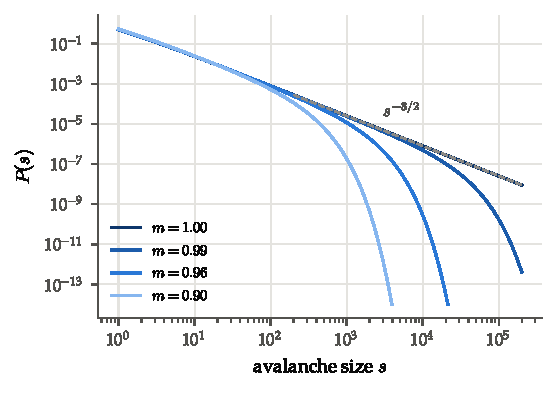
\includegraphics[width=0.55\linewidth]{theory/branching.pdf}
  \caption{Size distribution of the binary branching process for four values of the branching ratio $m$, from the exact result with the Catalan numbers
  \cref{eq:catalan}. Dashed: the critical power law $\sqrt{2/\pi}\,s^{-3/2}$.}
  \label{fig:branching}
\end{figure}

\subsection{Application to the sandpile limit}

In the fixed-drop sandpile of Chapter~\ref{ch:mapping}, a toppling sheds the force $\Delta f$, of which a fraction $1-\epsilon$, with
$\epsilon = 1/(2\ell^2+1)$, goes to the two neighbours. To turn this into a branching ratio we make the mean-field assumption that the forces of the
sites are spread uniformly over the interval of width $\Delta f$ below the threshold. A site that receives a force $\delta$ then topples with
probability $\delta/\Delta f$, and the expected number of topplings caused by one toppling is
\begin{equation}
  m = \frac{(1-\epsilon)\,\Delta f}{\Delta f} = 1-\epsilon = \frac{2\ell^2}{2\ell^2+1}.
\end{equation}
The sandpile limit is therefore a \emph{subcritical} branching process, below the critical point by exactly the bulk dissipation. The mean-field
predictions follow from \cref{eq:bp-mean,eq:bp-cutoff}:
\begin{equation}
  \avg{s} = \frac1\epsilon = 2\ell^2+1,\qquad s_c = \frac{2}{\epsilon^2}\approx 8\ell^4,
  \qquad P(s)\propto s^{-3/2}\ \text{for}\ s\ll s_c .
  \label{eq:bp-sandpile}
\end{equation}
For $\ell=6$ this predicts a power law with $\tau = 3/2$ over about four decades, up to $s_c\approx10^4$ topplings.

To test this we use the sandpile with random thresholds (noise width $w = 0.2$) of Chapter~\ref{ch:mapping}; without noise the sandpile is periodic
and has no meaningful statistics. The measured mean sizes are $\avg{s}/\ell^2 = \thsandSsix$ for $\ell=6$ and $\thsandStwelve$ for $\ell = 12$, close to
the prediction $(2\ell^2+1)/\ell^2\approx2.0$. The mean-field theory therefore gets the mean right. It gets the \emph{shape} wrong
(\cref{fig:sandpile-scaling}, right): below the cutoff, $P(s)$ decreases with an effective exponent of only $\tau_{\text{eff}}\approx\thsandTausix$, not $3/2$, and the
cutoff lies at a few tens of $\ell^2$ rather than near $8\ell^4$: nearly ten times lower than predicted for $\ell=6$, and more than twenty times lower for $\ell = 12$. The mean is
fixed by force balance and is insensitive to how the topplings are arranged; the shape is not, and the arrangement is what the branching process gets wrong.

% ======================================================================
\section{A one-dimensional approximation: random walk with losses}
\label{sec:th-randomwalk}

The failure of mean-field theory is a consequence of the dimension. On a chain, the offspring of a toppling are its two neighbours, and the
neighbours of those are again the original site and the sites next to it. Branches meet constantly, the same sites topple many times in one
avalanche, and the avalanche stays a compact interval. The random-walk picture of \cref{sec:mean} describes this geometry better.

Follow a packet of force $\Delta f$ released by a toppling. It is passed to a neighbour, which (when it topples in turn) passes it on, and at every
step the fraction $\epsilon$ is lost into the pulling spring. In the simplest version of this picture we let the whole packet survive each step with
probability $1-\epsilon$ and choose the next site at random among the two neighbours. Then:
\begin{enumerate}
  \item The packet survives $t$ steps with probability $(1-\epsilon)^t\approx e^{-\epsilon t}$, so it makes on average $1/\epsilon$ steps. Each
    step is a toppling, so the number of topplings per avalanche is of order $1/\epsilon = 2\ell^2+1$, as in mean-field theory.
  \item A random walk of $t$ steps covers a distance of order $\sqrt t$. During its lifetime the packet therefore visits an interval of length of
    order $\epsilon^{-1/2} = \sqrt{2\ell^2+1}\approx\sqrt2\,\ell$. This is the \emph{area} $a$ of the avalanche, the number of distinct sites
    that topple.
\end{enumerate}
The only length in this picture is $\ell$, and the only number of steps is $\ell^2$. If the approximation is right, the distributions of area and
size must therefore have the scaling forms
\begin{equation}
  P(a) = \frac1\ell\,F\!\left(\frac a\ell\right),\qquad P(s) = \frac1{\ell^2}\,G\!\left(\frac s{\ell^2}\right),
  \label{eq:rw-scaling}
\end{equation}
with functions $F$ and $G$ that do not depend on $\ell$. This is a sharp test: plotted as $\ell P(a)$ against $a/\ell$ and as $\ell^2P(s)$ against $s/\ell^2$,
the data for different $\ell$ must fall on one curve.

\Cref{fig:sandpile-scaling} shows that they do. For $\ell = 6$ and $\ell = 12$ the area distributions coincide over six decades, with an exponential tail
$P(a)\propto e^{-a/(\thsandDecaysix\,\ell)}$, and the mean area is $\thsandAsix\,\ell$ and $\thsandAtwelve\,\ell$, close to the estimate $\sqrt2\,\ell$. The size
distributions coincide in the bulk, and the extreme tail extends only slightly further for $\ell=12$. The noisy sandpile limit is therefore
described by a single scale, $\ell$ in space and $\ell^2$ in number of topplings, with no power law wider than about two decades in between. This
confirms quantitatively the conclusion of Chapter~\ref{ch:mapping}: the avalanches of the sandpile limit are confined to a few stiffness lengths by the
bulk dissipation.

\begin{figure}[t]
  \centering
  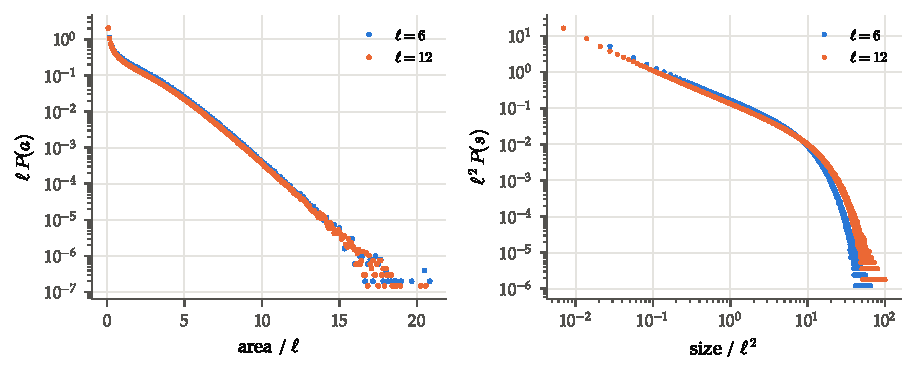
\includegraphics[width=\linewidth]{theory/sandpile_scaling.pdf}
  \caption{Scaling of the noisy sandpile limit (fixed-drop rule, $w = 0.2$) with the stiffness ratio $\ell$, as predicted by the random walk with losses
  \cref{eq:rw-scaling}. Left: number of distinct sites that topple (area). Right: number of topplings (size).}
  \label{fig:sandpile-scaling}
\end{figure}

% ======================================================================
\section{Inertial amplification in the BK model}
\label{sec:th-amplification}

\subsection{A rigid group with velocity weakening}

The sandpile is subcritical because every toppling sheds the same force, however many neighbours are also slipping. In the BK model this is not true.
\Cref{sec:one-block-event} computed the slip of a rigid group of $n$ blocks without velocity weakening; we now repeat the calculation with it.

Consider $n$ neighbouring blocks, all at threshold, that slip together by the same amount $\delta(\tau)$, while the blocks outside the group are stuck.
As in \cref{sec:one-block-event}, the spring force per block changes by $-\Omega_n^2\,\delta$ with
\begin{equation}
  \Omega_n^2 = 1+\frac{2\ell^2}{n}:
\end{equation}
the $n$ pulling springs and the two coupling springs at the ends of the group resist the motion, while the coupling springs inside the group are not
stretched. Friction is $\phi(2\alpha\dot\delta)$. With the 1991 law, $\phi(y) = (1-\sigma)/[1+y/(1-\sigma)]$, which for small velocities is
$\phi\approx(1-\sigma)-2\alpha\dot\delta$. The equation of motion per block is
\begin{equation}
  \ddot\delta = 1 - \Omega_n^2\,\delta - \phi(2\alpha\dot\delta)
  \quad\approx\quad
  \sigma - \Omega_n^2\,\delta + 2\alpha\,\dot\delta ,
  \qquad \delta(0) = \dot\delta(0) = 0 .
  \label{eq:group}
\end{equation}
This is the one-block equation of \cref{sec:one-block-event} with $\omega_1$ replaced by $\Omega_n$. The solution is therefore the same, and the slip per
block at the moment the velocity returns to zero is
\begin{equation}
  \delta_n = \frac{\sigma}{\Omega_n^2}\left(1+e^{\pi\alpha/\omega_n}\right),\qquad \omega_n = \sqrt{\Omega_n^2-\alpha^2}.
  \label{eq:group-slip}
\end{equation}

\subsection{Amplification and runaway}

\Cref{eq:group-slip} contains two sources of growth with $n$. The first is the factor $1/\Omega_n^2$: a longer group is held back by fewer coupling springs per
block. This is present without velocity weakening and gives $M_n\propto n^2$ for small groups (\cref{eq:Mn}). The second is the factor $e^{\pi\alpha/\omega_n}$:
the negative damping $2\alpha\dot\delta$ acts for the duration $\pi/\omega_n$ of the slip, and a longer group oscillates more slowly, so its slip is amplified
for longer. As $n$ grows, $\Omega_n$ decreases from $\omega_1 = \sqrt{2\ell^2+1}$ towards 1, and if $\alpha>1$ it reaches $\alpha$ at a finite group size:
\begin{equation}
  \Omega_{n^*}^2 = \alpha^2\quad\Longleftrightarrow\quad n^* = \frac{2\ell^2}{\alpha^2-1}.
  \label{eq:nstar}
\end{equation}
At $n = n^*$ the frequency $\omega_n$ vanishes and \cref{eq:group-slip} diverges. For $n>n^*$ the solutions of the linear equation \cref{eq:group} no longer
oscillate: both characteristic rates $\alpha\pm\sqrt{\alpha^2-\Omega_n^2}$ are real and positive, and the velocity grows exponentially without returning to
zero. In the linear approximation the group \emph{runs away}. In reality the slip is stopped by the nonlinearity of the friction law: as the velocity grows, friction
falls towards zero, and the group swings like an undamped oscillator about its new equilibrium. Its slip is then of order $2/\Omega_n^2$, i.e.\ of order one,
instead of order $\sigma$. We call $n^*$ the \emph{runaway size}. For $\ell = 6$ it is 9 blocks for $\alpha = 3$, 58 blocks for $\alpha=1.5$, and infinite
for $\alpha\le1$: with weak velocity weakening no group, however long, runs away.

Solving the full nonlinear equation \cref{eq:group} numerically confirms this picture. For $\ell=6$, $\alpha=3$ the slip per block is $6\times10^{-4}$ for one
block, $0.06$ at $n = n^* = 9$, and saturates at $1.5$ for very long groups: a factor of more than 2000 between a single block and a long group. For $\alpha = 1$ the
corresponding values are $3\times10^{-4}$, $0.004$ and $0.5$, and the growth is much more gradual.

\subsection{Comparison with the simulations}

A real event is not a rigid group: its blocks do not all start at threshold and do not all start at the same moment. The rigid group should therefore be read as an
upper estimate of the slip per block. \Cref{fig:amplification} compares it with the BK simulation for $\ell = 6$, $\alpha = 3$: for every event we compute the slip
per block, $M/n$, where $n$ is the number of blocks that slipped, and plot its median for each $n$. From $n = 1$ to $n = 8$ the slip per block grows by a factor
$\thampBK$ in the BK model and by $\thampRigid$ for the rigid group. The amplification is real and large, though weaker than for the idealised rigid group.

The sandpile limit behaves differently. Without noise every toppling is a slip of $\Delta f/(2\ell^2+1)$, so the slip per block equals the one-block value for every
event (dotted line). With noise a site can topple several times in one avalanche, and the slip per block grows by a factor $\thampSand$ from $n = 1$ to 8, but only because
of these repeated topplings; it never approaches the BK values. This is the missing ingredient identified in Chapter~\ref{ch:mapping}, now made quantitative: in the BK model
the force a slipping region passes to its surroundings grows with its size, so in the language of \cref{sec:th-branching} the effective branching ratio of an event
\emph{increases} as the event grows, from the subcritical value $1-\epsilon$ for a single block to a supercritical value once the slipping region exceeds $n^*$.

\begin{figure}[t]
  \centering
  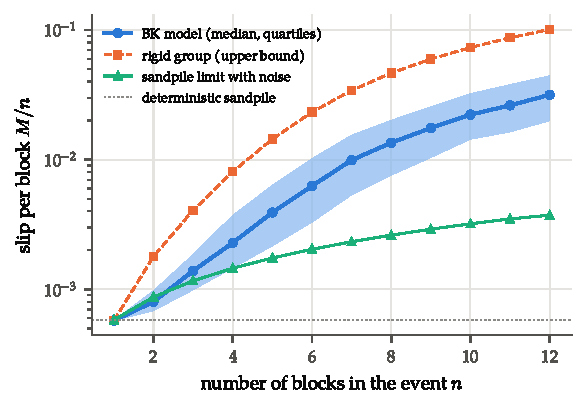
\includegraphics[width=0.62\linewidth]{theory/amplification.pdf}
  \caption{Slip per block as a function of the number of blocks in the event ($\ell=6$, $\alpha=3$, $\sigma=0.01$). BK model: median and quartiles over all events
  with $n$ blocks. Rigid group: numerical solution of \cref{eq:group}. Sandpile: fixed-drop rule with $\Delta f$ from \cref{eq:map-drop}, with noise $w = 0.2$ and
  without noise.}
  \label{fig:amplification}
\end{figure}

% ======================================================================
\section{When are there great events?}
\label{sec:th-bimodal}

\subsection{A criterion}

The size distributions of the BK model have a separate peak of great (delocalized) events for $\alpha = 3$, but not for $\alpha = 1$
(\cref{fig:alpha-test}). The runaway size suggests why. An event that is still localized can turn into a great event only if its slipping region becomes longer than
$n^*$; below that size every slip is stopped by the springs. The localization length $\tilde\xi$ of Carlson \emph{et al.} (\cref{eq:xi-tilde}) is the size of the largest
triggering zone that a growing pulse can cross without breaking out. Combining the two:
\begin{itemize}
  \item if $n^*<\tilde\xi$, localized events reach the runaway size before they reach the end of their zone, and some of them run away: there is a separate population of
    great events;
  \item if $n^*>\tilde\xi$, localized events die out before they become long enough to run away, events grow gradually, and the distribution has no separate peak;
  \item for $\alpha\le1$, $n^* = \infty$ and there are no great events in this sense for any $\ell$.
\end{itemize}
The criterion $n^*<\tilde\xi$ involves both parameters. With $n^* = 2\ell^2/(\alpha^2-1)$ and $\tilde\xi = (2\ell/\alpha)\ln(4\ell^2/\sigma)$, the ratio
\begin{equation}
  \frac{n^*}{\tilde\xi} = \frac{\alpha\,\ell}{(\alpha^2-1)\ln(4\ell^2/\sigma)}
  \label{eq:bimodal}
\end{equation}
grows with $\ell$. At fixed $\alpha$, a stiffer chain therefore needs stronger velocity weakening to produce great events. This is a prediction that a criterion based on
$\alpha$ alone would not make.

\subsection{Measuring bimodality}

To test the criterion we need a measure of how strongly the great events are separated from the localized ones. We use the \emph{depth of the minimum}: the difference
between $\ln\mathcal D(\mu)$ at the peak of the great events and at the minimum to its left (both after averaging over bins of width 0.5 in $\mu$). A positive depth means
the distribution falls, reaches a minimum and rises again; a depth of zero or below means it decreases monotonically. This depth also grows with the width of the
localized power law, so it measures the existence of a separate population, not its strength in a way that can be compared between different values of $\ell$.

We ran the BK model for ten values of $\alpha$ between 1 and 5 at $\ell = 6$ ($N = 4096$, 500 units of plate displacement each), and for $\alpha = 1.25$, 1.5, 1.75
and 2 at $\ell=12$ ($N = 8192$, 300 units). Together with the runs of Chapters~\ref{ch:mapping} and~\ref{ch:results} at $\alpha = 1$ and $\alpha = 3$, these cover
values of $n^*/\tilde\xi$ from about 0.1 to infinity.

\subsection{Results}

\Cref{fig:alpha-scan} shows the distributions at $\ell = 6$. The change with $\alpha$ is gradual for small events and abrupt for large ones. For $\alpha = 1$ and $1.25$ the
distribution of moments decreases monotonically up to the cutoff, and the distribution of the number of blocks per event is a single smooth curve. From $\alpha = 1.35$ on, a
minimum appears near $M\approx\xi$ and a separate peak of great events at $M\approx30\,\xi$, and in the distribution of blocks a plateau of events with several hundred blocks
separates from the rest. For $\alpha\ge2.5$ the shape hardly changes any more.

\begin{figure}[t]
  \centering
  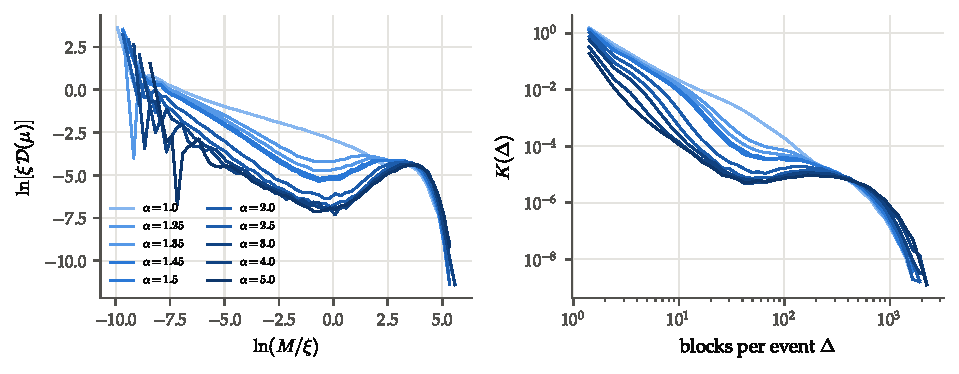
\includegraphics[width=\linewidth]{theory/alpha_scan.pdf}
  \caption{The BK model for $\alpha$ from 1 to 5 ($\ell=6$, $\sigma=0.01$, $N=4096$). Left: frequency per unit magnitude. Right: frequency of events with $\Delta$
  blocks, per unit length and unit plate displacement.}
  \label{fig:alpha-scan}
\end{figure}

\Cref{tab:bimodal} and the middle panel of \cref{fig:crossover} compare the depth of the minimum with the criterion. At $\ell = 6$ the agreement is good: the criterion
$n^* = \tilde\xi$ predicts the onset of great events at $\alpha = \thonsetsix$, and the simulations show no minimum at $\alpha = 1.25$ ($n^*/\tilde\xi = 1.39$) and a clear one from
$\alpha = 1.35$ ($n^*/\tilde\xi = 1.03$) on. Its depth then grows steadily and saturates for $\alpha\gtrsim2.5$.

At $\ell = 12$, however, the criterion fails. It predicts that the onset moves to $\alpha = \thonsettwelve$, because $n^*$ grows as $\ell^2$ while $\tilde\xi$ grows only as
$\ell\ln\ell$. The simulations show the opposite: at $\ell = 12$ a minimum is already present at $\alpha = 1.5$ ($n^*/\tilde\xi = 1.31$), with the same depth as at $\ell = 6$, and a
shallow one even at $\alpha = 1.25$ ($n^*/\tilde\xi = 2.43$). At fixed $\alpha$ the minimum is at least as deep for $\ell=12$ as for $\ell = 6$, and for $\alpha = 3$ it deepens steadily
from $\ell = 6$ to $\ell = 24$, where the criterion predicts that it should become shallower. The onset of great events therefore moves to \emph{smaller} $\alpha$ as $\ell$ grows,
not to larger $\alpha$.

The test thus refutes the criterion $n^*<\tilde\xi$ as a description of the dependence on $\ell$; its success at $\ell = 6$ is a coincidence of the numerical prefactors. What
survives is the weaker statement that great events require $\alpha>1$. The runs with $\alpha = 1$ ($\ell = 6$, 10 and 14), for which no finite group runs away, show no minimum or
only a trace of one (depth $\le0.1$), and the onset at finite $\ell$ lies somewhat above $\alpha = 1$ and approaches it as $\ell$ grows. This is consistent with the runaway of a
long group, $\Omega_\infty = 1<\alpha$, being the mechanism of the great events, but it shows that the size at which an event runs away is not $n^*$ of the rigid-group
calculation. A real event is not rigid: its slipping region is a pair of pulses that move outward, and the coupling springs inside it are stretched, so the restoring force per
block is not $\Omega_n^2$. A better estimate of the runaway size would have to start from the pulse solution of \cref{sec:bk-pulses} rather than from a rigid group.

\begin{table}[t]
\centering
\caption{Runaway size $n^*$ (\cref{eq:nstar}), localization length $\tilde\xi$ (\cref{eq:xi-tilde}) and depth of the minimum of $\mathcal D(\mu)$ for all runs with
$\sigma=0.01$. A depth of zero or below means that there is no separate population of great events.}
\label{tab:bimodal}
\begin{tabular}{cccccc}
\toprule
$\ell$ & $\alpha$ & $n^*$ & $\tilde\xi/a$ & $n^*/\tilde\xi$ & depth \\
\midrule
\tabinput{figures/theory/dip_table.tex}
\bottomrule
\end{tabular}
\end{table}

% ======================================================================
\section{The crossover moment}
\label{sec:th-crossover}

Carlson \emph{et al.} estimate that the localized events end at the crossover moment $\tilde M = 2\xi/\alpha$ (\cref{eq:M-tilde}): proportional to the stiffness
length $\xi$, inversely proportional to $\alpha$, and independent of $\sigma$. Chapter~\ref{ch:results} confirmed the independence of $\sigma$. To test the other two
dependences we need a definition of the crossover that can be applied to every run. We use the moment $M_c$ at which the effective exponent of $P(M)$, measured in
windows $[M,10M]$, first falls below 1. Since $\mathcal D(\mu) = M\,P(M)$, an effective exponent of 1 means that $\mathcal D(\mu)$ is locally flat, so $M_c$ is the
point where $\mathcal D(\mu)$ stops decreasing; it coincides with the minimum of $\mathcal D(\mu)$ when there is one, and it remains defined when there is not.

\Cref{fig:crossover} (left) shows $M_c$ for the $\alpha$-scan at $\ell=6$. For all $\alpha$ between 1.25 and 5, $M_c$ lies between $\thMcMin\,\xi$ and $\thMcMax\,\xi$, without a
trend; the prediction $2\xi/\alpha$ decreases by a factor of four over the same range. The right panel shows $M_c$ for $\alpha = 3$ and $\ell$ from 6 to 24. The prediction
$\tilde M/\xi = 2/3$ is independent of $\ell$; the measured ratio falls from $\thMcXiLsix$ at $\ell = 6$ to $\thMcXiLtwentyfour$ at $\ell = 24$, because $M_c$ itself stays between
$\thMcLmin\,a$ and $\thMcLmax\,a$ while $\xi$ grows by a factor of four. The direct positions of the minimum of $\mathcal D(\mu)$ tell the same story: they lie at
$M\approx3.5$--$6\,a$ for all five values of $\ell$.

Neither dependence of $\tilde M$ is therefore confirmed. Within the parameter range studied ($\ell\le24$), the crossover from localized to delocalized events happens at a
moment of a few units of $a$, nearly independent of $\alpha$, $\sigma$ and $\ell$. The estimate $\tilde M = 2\xi/\alpha$ has the right order of magnitude for $\ell = 6$, which
is the case Carlson \emph{et al.} studied most, but not the right scaling. It is based on the linear pulse equation, which describes a single pulse growing in a uniform
region at threshold; the crossover in the simulations is instead set by events that start in the rough configurations left by earlier events, which that calculation does
not describe. We have not found an approximate theory for the position of the crossover, and we leave it as an open question.

\begin{figure}[t]
  \centering
  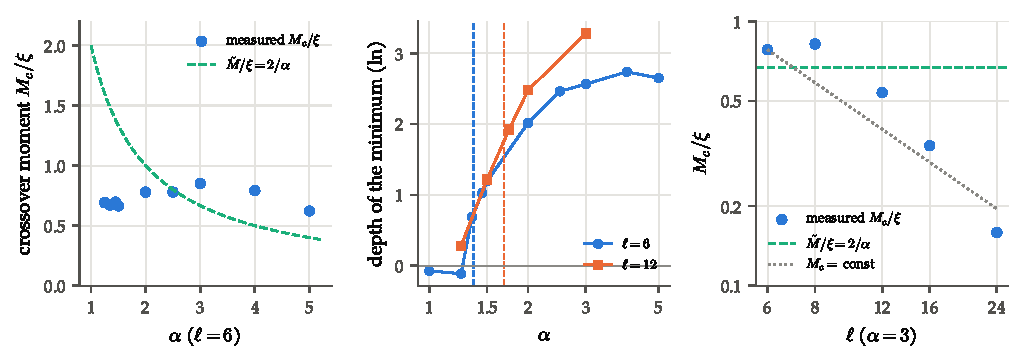
\includegraphics[width=\linewidth]{theory/crossover.pdf}
  \caption{Tests of the approximate theory. Left: crossover moment against $\alpha$ ($\ell=6$), with the prediction $\tilde M = 2\xi/\alpha$. Middle: depth of the minimum of
  $\mathcal D(\mu)$ against the ratio of the runaway size and the localization length, \cref{eq:bimodal}; runs with $\alpha\le1$ ($n^*=\infty$) are plotted at the right
  edge. Right: crossover moment against $\ell$ ($\alpha=3$), with the prediction and the line of constant $M_c$.}
  \label{fig:crossover}
\end{figure}

% ======================================================================
\section{The exponent of the localized events}
\label{sec:th-exponent}

The last question is whether any of these approximations predicts the exponent of the localized power law. \Cref{tab:alpha} gives the exponent from
maximum-likelihood fits between $\max(10M_1, 10^{-4}\xi)$ and $10^{-2}\xi$ for the $\alpha$-scan at $\ell = 6$. It is not a constant: $\tau$ rises from about 1.5 at
$\alpha=1$ to a maximum of about 1.97 at $\alpha = 3$ and decreases again for larger $\alpha$.

\begin{table}[t]
\centering
\caption{The $\alpha$-scan at $\ell=6$: exponent $\tau$ of the localized region, crossover moment $M_c$, runaway size $n^*$ and localization length $\tilde\xi$.}
\label{tab:alpha}
\begin{tabular}{ccccc}
\toprule
$\alpha$ & $\tau$ & $M_c/\xi$ & $n^*$ & $\tilde\xi/a$ \\
\midrule
\tabinput{figures/theory/alpha_table.tex}
\bottomrule
\end{tabular}
\end{table}

Two conclusions follow. First, the localized events are not a critical branching process: mean-field theory predicts the universal value $\tau = 3/2$ at its critical point,
whereas the measured exponent depends continuously on a parameter of the friction law and lies well above $3/2$ for the values studied by Carlson \emph{et al.} The value near
$3/2$ at $\alpha=1$ should not be taken as a confirmation: at $\alpha=1$ the effective exponent drifts slowly over the whole range (Chapter~\ref{ch:mapping} found $\tau\approx1.4$
in a different window), and the branching process has no reason to apply there either. Second, an exponent that varies continuously with a model parameter is not a universal
critical exponent in the sense of \cref{sec:critical}. Such non-universal exponents are known from the OFC model, whose exponent depends on the degree of conservation, and they are
another sign that the BK model is not critical in the strict sense. In the picture of \cref{sec:bk-events}, the localized events smooth the rough configurations left by great
events, so their statistics are inherited from the roughness of these configurations, which depends on how strongly the great events amplify irregularities, i.e.\ on $\alpha$.
Turning this picture into a calculation of $\tau$ would require a theory of the roughness, which we have not attempted.

% ======================================================================
\section{Summary}
\label{sec:th-summary}

\begin{enumerate}
  \item \textbf{Mean field.} The branching process gives $\tau=3/2$ at its critical point, a cutoff $s_c\propto(1-m)^{-2}$ and a mean size $(1-m)^{-1}$. The sandpile limit of the BK
    model is a subcritical branching process with $m = 1-\epsilon = 2\ell^2/(2\ell^2+1)$. Mean-field theory predicts its mean avalanche size correctly, but not the shape of the
    distribution.
  \item \textbf{Random walk with losses.} In one dimension the appropriate approximation is a random walk that loses the fraction $\epsilon$ at each step. It predicts that the noisy
    sandpile limit has a single scale, $\ell$ in space and $\ell^2$ in number of topplings, and the simulations collapse accordingly. The sandpile limit is not critical for any $\ell$.
  \item \textbf{Amplification.} A rigid group of $n$ blocks with velocity weakening slips by an amount that grows rapidly with $n$ and runs away above $n^* = 2\ell^2/(\alpha^2-1)$.
    The simulations show this amplification, weaker than for the rigid group, and the sandpile limit lacks it. This makes quantitative the failure of the mapping found in
    Chapter~\ref{ch:mapping}.
  \item \textbf{Great events.} A separate population of great events exists only for $\alpha>1$, as the runaway of long groups requires. The criterion $n^*<\tilde\xi$, which
    combines the rigid-group runaway size with the localization length, predicts the onset correctly at $\ell = 6$ ($\alpha\approx1.3$) but fails at $\ell = 12$: the onset moves to
    smaller $\alpha$ as $\ell$ grows, not to larger.
  \item \textbf{Crossover and exponent.} The crossover moment is not described by $\tilde M = 2\xi/\alpha$: it stays at a few units of $a$ for all $\alpha$ and $\ell$ studied. The exponent
    of the localized region varies with $\alpha$ and is not the mean-field value. Neither is explained by the approximations of this chapter.
\end{enumerate}
